\section{Reconstructing the black hole from the boundary, outside the horizon \label{sec:outside}}

We will now try to reconstruct the black hole geometry from the boundary. 
In AdS/CFT we have the following identifications between the boundary CFT and the bulk
\[
\begin{split}
{\rm Thermalization\,\,of\,\,pure\,\,state} &\qquad\Leftrightarrow\qquad 
{\rm Black\,\, hole\,\, formation\,\, by\,\, gravitational\,\, collapse}\cr
{\rm Thermal\,\, density\,\, matrix}  & \qquad\Leftrightarrow\qquad {\rm Eternal\,\, black\,\, hole}
\end{split}
 \]
In the same way that the collapsing star can be approximated  {\it for certain questions} by the eternal black hole, we expect that late time\footnote{As in the bulk, by late we mean after the thermalization has occurred, but not too late so that Poincare recurrences and other finite $N$ effects become important.} CFT correlation functions on a heavy pure state can be approximated by correlation functions on a thermal density matrix. 

Hence, we will first focus on thermal correlators and explain how to represent local bulk operators in the case where the boundary theory is in a thermal density matrix. We will then carry over this definition of the operator (at large $N$) to the case where we have a typical pure state. We will discuss the validity of this approach and possible non-trivial sensitivity on the specific pure state in section \ref{sec:subtleties}.




\subsection{Boundary thermal correlators}


\subsubsection{Large $N$ factorization at finite $T$}
\label{factorcav}

Let us consider a scalar conformal primary operator ${\cal O}$. For simplicity we assume that its thermal 1-point function ${\rm Tr}(\rho \,{\cal O})$ vanishes,  
where $\rho = e^{-\beta H}$. This can be ensured by considering a theory with a ${\mathbb Z}_2$ symmetry, under which ${\cal O}$ is odd.

A central assumption in what follows is that large $N$ factorization holds for thermal correlation functions i.e. that we have the analogue of \eqref{factorization}
\[
{\rm Tr}(\rho \,{\cal O}(x_1)...{\cal O}(x_{2n})) = {1\over 2^n} \sum_\pi
{\rm Tr}(\rho \,{\cal O}(x_{\pi_1}) {\cal O}(x_{\pi_2}))...{\rm Tr}(\rho \,{\cal O}(x_{\pi_{2n-1}}) {\cal O}(x_{\pi_{2n}})) + \ldots,
\]
where the dots are terms that are subleading in ${1 \over N}$. 
Of course the 2-point function ${\rm Tr}(\rho\, {\cal O}(x_1)\, {\cal O}(x_2))$ in which the thermal correlators factorize into is completely different 
from the zero temperature 2-point function $\lvac {\cal O}(x_1) {\cal O}(x_2) \rvac$. Also, we need to stress that ---as in the zero temperature case---
there are several caveats about the validity of factorization. We should be careful to {\it first} fix all other parameters/numbers that enter the correlator and {\it then} take $N$ to infinity. For example, factorization can fail if

\begin{itemize}
\item We scale the number of operators (i.e. $n$ in the formula above) with some power of $N$. Scaling the number of external legs with powers of $N$ invalidates the naive 't Hooft counting and a priori we have no reason to expect the correlator to still factorize.

\item We scale the conformal dimension of ${\cal O}$ in an $N$-dependent way --- the same comments as above apply.

\item We scale some of the distances $|x_i-x_k|$ to be too small, in an $N$-dependent way (this can be thought of as a high energy scattering, where higher and higher loops in $1/N$ become important).

\item We scale the temperature in a $N$-dependent way. (See the paragraph in section \ref{secadseternal} for more details.)

\item We scale (some of) the distances $|x_i-x_j|$ to {\it increase} in an $N$-dependent fashion. This will be particularly important when we consider the operators evaluated on
typical pure states vs the thermal ensemble.

\end{itemize}
Of course this list is not supposed to be exhaustive. In general we have to be careful about how various factors in the problem scale, when taking the large $N$ limit.



\subsubsection{Analytic structure of thermal 2-point functions}
\label{therman}

We now discuss general properties on finite temperature Wightman functions. Since correlators at large $N$ factorize to products of 2-point functions, we will focus on the latter. 

Consider two local operators ${\cal O}_1,{\cal O}_2$. From time and space translational invariance of the thermal ensemble we only need
\[
F_{12}(t) \equiv Z_{\beta}^{-1}{\rm Tr}\left(e^{-\beta H} {\cal O}_1(t,\vect{x}) \, {\cal O}_2(0,\vect{0})\right),
\]
where we did not indicate the $\vect{x}$ dependence on the LHS. Here 
\[
Z_{\beta} = {\rm Tr}\left[e^{-\beta H}\right],
\]
 is the partition function which will appear frequently below. Since the operators do not generally commute, we also have a related function
\[
F_{21}(t) \equiv Z_{\beta}^{-1}{\rm Tr}\left(e^{-\beta H} {\cal O}_2(0,\vect{0}) \, {\cal O}_1(t,\vect{x})\right).
\]
Let us keep $\vect{x}$ fixed and analytically continue $t$ to complex values. By inserting a complete set of states and using the positivity of the energy spectrum we find that the analytically continued function $F_{12}(t)$ is meromorphic in the strip
\[
-\beta<{\rm Im}\,t <0.
\]
However, in general, it cannot be analytically continued to positive values of ${\rm Im}\,t$.  The function $F_{21}(t)$ can be analytically continued to positive imaginary values of $t$ and is meromorphic in the strip 
\[
0<{\rm Im} \,t<\beta.
\]  

The value of the function $F_{12}(t)$ for real $t$ is equal to the limit of the meromorphic function in the strip $-\beta<{\rm Im}t <0$, as we take ${\rm Im} t \rightarrow 0^-$ from below. As we approach the other end of the strip from above (i.e. ${\rm Im}t \rightarrow -\beta^-$) and by inserting a complete set of states and using the cyclicity of the trace we derive the so called KMS condition
\be
\label{kms}
F_{12}(t-i\beta^-) = F_{21}(t).
\ee
So the correlator is periodic in imaginary time, up to an exchange in the order of the insertion of operators. 

The discussion so far has been very general and would apply to any quantum system at finite temperature, even in non-relativistic quantum mechanics. In relativistic QFT we have an important additional property: local operators at spacelike separation commute. This means that the functions $F_{12}(t)$ and $F_{21}(t)$ must have the same value along the segment of the real axis $-|\vect{x}|<t<|\vect{x}|$ and hence one must be the analytic continuation of the other! For $t>|\vect{x}|$ we generally have $\lim_{{\rm Im}\, t\rightarrow 0^-} F_{12}(t) \neq \lim_{{\rm Im}\, t\rightarrow 0^+} F_{21}(t)$ and this discontinuity is proportional to the (thermal expectation value of the) commutator of the two operators. Because of the KMS condition this discontinuity appears periodically along all semi-infinite lines $t = \pm (|\vect{x}| + {\cal R}^+) + i m \beta$ where ${\cal R}^+$ denotes positive real numbers and $m \in \mathbb{Z}$.

Hence, by combining the KMS condition with the spacelike commutativity of local fields we have arrived at the following important conclusion: consider the domain ${\cal D}$ of the complexified $t$-plane defined as $\mathbb{C}$ minus ``cuts'' starting from $\pm|\vect{x}| + i m \beta$ and extending all the way to infinity parallel to the real axis, as depicted in figure \ref{analyticity}. This domain ${\cal D}$ is a simply-connected domain. Then, there is a {\it holomorphic} function ${\cal F}(z)$ defined in the domain ${\cal D}$ with the property that
\[
{\cal F}(z+i\beta) = {\cal F}(z) ,
\]
for all $z\in {\cal D}$ and also
\begin{align}
\nonumber
\lim_{\epsilon \rightarrow 0^+} {\cal F}(t-i \epsilon) = F_{12}(t), \\
\nonumber
\lim_{\epsilon \rightarrow 0^+} {\cal F}(t+i \epsilon) = F_{21}(t).
\end{align}
The holomorphic function ${\cal F}$ contains all the information about the 2-point function of operators ${\cal O}_1,{\cal O}_2$ for both possible orderings.
\begin{figure}
\begin{center}
\psfrag{beta}{$\beta$}
\psfrag{beta2}{$2\beta$}
\psfrag{beta3}{$-\beta$}
\psfrag{beta4}{$-2\beta$}
\psfrag{Ret}{${\rm Re}(t)$}
\psfrag{zero}{$0$}
\psfrag{xplus}{$|\vect{x}|$}
\psfrag{xminus}{$-|\vect{x}|$}
\psfrag{Imt}{${\rm Im}(t)$}
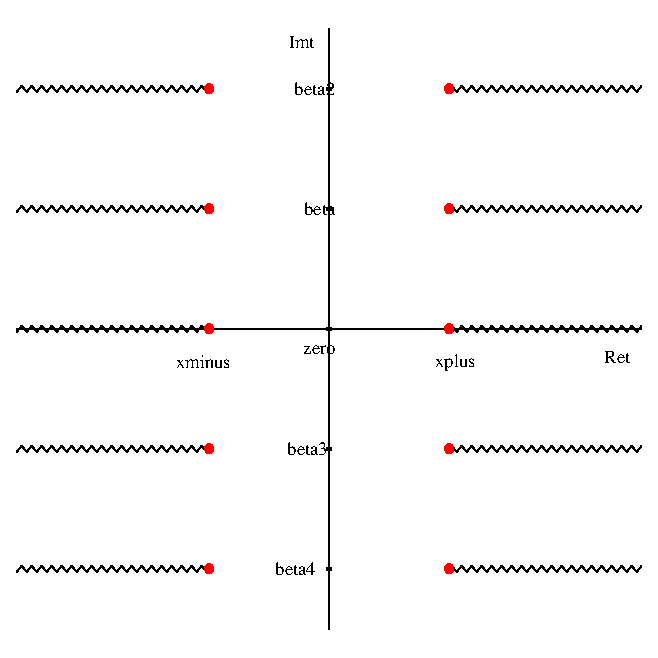
\includegraphics[width=9cm]{analyt.eps}
\caption{Domain of analyticity of a thermal 2-point function of the two local operators ${\cal O}_1(t,\vect{x})$ and ${\cal O}_2(0,\vect{0})$. The domain ${\cal D}$ is defined as the complex plane with the indicated branch cuts removed. On this domain we have a holomorphic function ${\cal F}(z)$ which satisfies ${\cal F}(z+i\beta)= {\cal F}(z)$. The function ${\cal F}$ contains all information about the thermal 2-point function. For example, we have $\lim_{\epsilon\rightarrow 0^+}{\cal F}(t-i\epsilon) = Z_{\beta}^{-1}{\rm Tr}\left(e^{-\beta H} {\cal O}_1(t,\vect{x}) {\cal O}_2(0,\vect{0})\right)$ and also 
 $\lim_{\epsilon\rightarrow 0^+}{\cal F}(t+i\epsilon) = Z_{\beta}^{-1}{\rm Tr}\left(e^{-\beta H} {\cal O}_2(0,\vect{0}){\cal O}_1(t,\vect{x}) \right)$
. The discontinuity along the branch cut is proportional to the thermal expectation value of the commutator of the two operators.}
\label{analyticity}
\end{center}
\end{figure}

We mentioned that generally $F_{12}(t)$ cannot  be analytically continued to complex $t$ with positive imaginary part by going through the part of the positive real axis with $t>|\vect{x}|$ (i.e. the analytic continuation is possible only by going around, and through the ``spacelike segment'' $-|\vect{x}|<t<|\vect{x}|$). While this is indeed  generic, it is not always true: there are quantum systems (for example a free QFT) whose thermal 2-point function {\it can} be analytically continued up through the part of the positive real axis with $t>|\vect{x}|$. However even in that case, the analytic continuation of the function through what used to be the ``cut'' of the domain ${\cal D}$ {\it does not lead to the same value} as the one that we would get by going through the ``spacelike segment'' which lies purely within the domain ${\cal D}$. In other words the correlation functions analytically continued to complex times are generically multivalued functions --- and we have to specify the ``sheet'' on 
which we are evaluating them.

We will define the ``principal sheet'' of the analytically continued thermal correlators, as the one defined by doing the continuation purely within the domain ${\cal D}$ described above. This will be very important when we discuss the analytic continuation behind the horizon. Let us emphasize this once more: whenever we write down a thermal correlator where some of the time arguments have been given an imaginary value, the {\it definition} of this analytically continued correlator is that one has to start with the correlator defined in ``real time'' and then continue it to the complex values by working only in the domain ${\cal D}$ and going ``around'' the cuts, through the Euclidean (spacelike) region. 

After these generalities, let us return to the case where we are looking at the thermal 2-point function of a conformal primary ${\cal O}$. From translational invariance in space and time we only need the function
\[
G_\beta(t,\vect{x}) = Z_{\beta}^{-1}{\rm Tr}\left(e^{-\beta H}{\cal O}(t,\vect{x})\,{\cal O}(0,\vect{0})\right),
\]
we will also consider its Fourier transform
\[
G_\beta(\omega,\vect{k}) = \int dt d^{d-1}\vect{x} \,\, e^{i \omega t - i \vect{k}
\vect{x}}\,G_{\beta}(t,\vect{x}).
\]
We have the following general properties. First, rotational invariance implies
\[
G_\beta(t,\vect{x}) = G_\beta(t,-\vect{x}).
\]
Second the KMS condition for the thermal trace implies
\[
G_{\beta}(t-i\beta,\vect{x}) = G_\beta(-t,-\vect{x}).
\]
In Fourier space the corresponding statements are
\[
G_\beta(\omega,\vect{k}) = G_\beta(\omega,-\vect{k}),
\label{rotfourier}
 \]
\[
G_\beta(-\omega,\vect{k}) = e^{-\beta \omega} G_\beta(\omega,\vect{k}).
\label{kmsfourier}
 \]
These are exact properties which hold in all dimensions and arbitrary coupling.\footnote{Clearly the discussion in this section was also independent of large $N$.} We can explicitly verify them in the case of 2d CFT thermal real-time correlation functions, which can be explicitly computed, as presented in appendix \ref{appendix2dthermal}. 

\subsubsection{Mode expansion of thermal 2-point function}

Now we proceed by expanding the boundary field in its Fourier modes. For simplicity we take the CFT to live in ${\mathbb R}^{d-1,1}$ at finite temperature.\footnote{We could also do a similar analysis for the finite temperature CFT on ${\mathbb S}^{d-1}\times {\rm time}$, where we would have to replace the ${\bf k}$ momenta with discrete spherical harmonic modes.} We have  
\be
\label{modesa}
{\cal O}(t,\vect{x}) = \int_{\omega>0} {d\omega d^{d-1}\vect{k} \over (2 \pi)^d} \,\,\left( {\cal O}_{\omega,\vect{k}} e^{-i\omega t +i \vect{k} \vect{x}} +  {\cal O}_{\omega,\vect{k}}^\dagger e^{i\omega t -i \vect{k} \vect{x}}\right) 
\ee
As before, this is the {\it definition} of the (non-local) operators ${\cal O}_{\omega,\vect{k}}$.

We can now consider the thermal 2-point function of ${\cal O}$ expanded in terms of its modes. From translational invariance we immediately conclude that
\[
Z_{\beta}^{-1}{\rm Tr}\left(e^{-\beta H} {\cal O}_{\omega,\vect{k}} {\cal O}_{\omega',\vect{k}'} \right) =  
Z_{\beta}^{-1}{\rm Tr}\left(e^{-\beta H} {\cal O}_{\omega,\vect{k}}^\dagger {\cal O}_{\omega',\vect{k}'}^\dagger \right) =0,
\]
and for the other combinations we have
\begin{align}
\nonumber 
&Z_{\beta}^{-1}{\rm Tr}\left(e^{-\beta H} {\cal O}_{\omega,\vect{k}} {\cal O}_{\omega',\vect{k}'}^\dagger \right)
= G_\beta(\omega,\vect{k}) \delta(\omega-\omega') \delta^{d-1}(\vect{k}-\vect{k}'), \\
\nonumber
&Z_{\beta}^{-1}{\rm Tr}\left(e^{-\beta H} {\cal O}_{\omega,\vect{k}}^\dagger {\cal O}_{\omega',\vect{k}'} \right)
= G_\beta(-\omega,-\vect{k}) \delta(\omega-\omega') \delta^{d-1}(\vect{k}-\vect{k}').
\end{align}
So for the thermal expectation value of the commutator we have
\[
Z_{\beta}^{-1}{\rm Tr}\left(e^{-\beta H} [{\cal O}_{\omega,\vect{k}}\,,\, {\cal O}_{\omega',\vect{k}'}^\dagger] \right)
= \left(G_\beta(\omega,\vect{k})- G_\beta(-\omega,-\vect{k}) \right)\delta(\omega-\omega') \,\delta^{d-1}(\vect{k}-\vect{k}').
\]


Actually, given large $N$ factorization of the thermal correlators we can derive a more general statement: the relations above hold even in the presence of other operators ${\cal T}_m$ even if they are ``composite'', as long as they are ``light'' and their scaling dimension does not scale with $N$:
\begin{align}
\nonumber
\tr\left(e^{-\beta H} {\cal T}_1 [{\cal O}_{\omega,\vect{k}}\,,\, {\cal O}_{\omega',\vect{k}'}] {\cal T}_2\right) =
&\tr\left(e^{-\beta H} {\cal T}_1[{\cal O}_{\omega,\vect{k}}^\dagger\,,\, {\cal O}_{\omega',\vect{k}'}^\dagger] {\cal T}_2\right)=0, \\
\label{thermalcoma}
\tr\left(e^{-\beta H} {\cal T}_1[{\cal O}_{\omega,\vect{k}}\,,\, {\cal O}_{\omega',\vect{k}'}^\dagger]  {\cal T}_2\right) 
= &\left(G_\beta(\omega,\vect{k})- G_\beta(-\omega,-\vect{k}) \right)\delta(\omega-\omega') \,\delta^{d-1}(\vect{k}-\vect{k}') \\ \nonumber &\times \tr\left(e^{-\beta H} {\cal T}_1 {\cal T}_2 \right).
 \end{align}

The commutator \eqref{thermalcoma} implies that the operators ${\cal O}_{\omega,\vect{k}}$ behave like the creation and annihilation operators of harmonic oscillators, though in an unconventional normalization. We can rescale them and define operators
\be
\label{rescaled}
\hatbb{\cal O}_{\omega,\vect{k}} = {{\cal O}_{\omega,\vect{k}} \over \left(
G_\beta(\omega,\vect{k})- G_\beta(-\omega,-\vect{k})\right)^{1\over 2}},
\ee
which have canonical commutation relations. If we compute the thermal expectation value of the ``occupation level'' $n_{\omega,\vect{k}}=\hatbb{\cal O}_{\omega,\vect{k}}^\dagger 
\hatbb{\cal O}_{\omega,\vect{k}} 
$ for each of these oscillators we have
\[
Z_{\beta}^{-1}{\rm Tr}\left( e^{-\beta H} \hatbb{\cal O}_{\omega,\vect{k}}^\dagger 
\hatbb{\cal O}_{\omega',\vect{k}'}\right) = { G_\beta(-\omega,
-\vect{k})\over G_\beta(\omega,\vect{k})- G_\beta(-\omega,-\vect{k})} \delta(\omega-\omega')\delta^{d-1}(\vect{k}-\vect{k}')
\]
and we find using \eqref{rotfourier} and \eqref{kmsfourier} that
\be
\label{thermaloca}
Z_{\beta}^{-1}{\rm Tr}\left( e^{-\beta H} \hatbb{\cal O}_{\omega,\vect{k}}^\dagger 
\hatbb{\cal O}_{\omega',\vect{k}'}\right)= {1\over e^{\beta \omega}-1} \delta(\omega-\omega')\delta^{d-1}(\vect{k}-\vect{k}'),
\ee
and similarly
\be
\label{thermalocab}
Z_{\beta}^{-1}{\rm Tr}\left( e^{-\beta H} \hatbb{\cal O}_{\omega,\vect{k}}
\hatbb{\cal O}_{\omega',\vect{k}'}^\dagger \right)= {e^{\beta \omega}\over e^{\beta \omega}-1} \delta(\omega-\omega')\delta^{d-1}(\vect{k}-\vect{k}'),
\ee
which is the standard occupation level for a harmonic oscillator of frequency $\omega$ when placed at temperature $\beta$. 

The physical interpretation of these results is that the modes \eqref{thermalcoma} are the CFT analogue of the AdS-Schwarzschild modes of a scalar field around a black hole in AdS that we called $a_{\omega,\vect{k}}$ in section \ref{modesbrane} hence we have the natural identification
\vskip5pt
\[
 \hatbb{\cal O}_{\omega,\vect{k}}\qquad\Leftrightarrow \qquad a_{\omega,\vect{k}}
\]
\vskip5pt
The CFT modes $\hatbb{\cal O}_{\omega,\vect{k}}$ seem to be thermally populated at the Hawking temperature of the black hole $\beta$, as we see in \eqref{thermaloca},\eqref{thermalocab}. This is the CFT analogue of the ``thermal atmosphere'' of the black hole that we discussed in the previous sections, for example in equations \eqref{hhocup}, \eqref{hhocupb}. In a sense, they can be thought of as a thermally excited gas of glueballs, hovering around the quark-gluon plasma --- though the interpretation
may be not fully accurate. More technically it means that, as expected, we get the occupation levels determined by the AdS-Hartle-Hawking vacuum for the dual scalar field. It is interesting that this result follows simply from general properties of thermal field theories {\it together with large $N$ factorization} and does not need any other assumptions about the coupling. In particular the same conclusion would hold for the regime of small $\lambda$ where 
the spacetime and the dual black hole would be highly stringy. On the other hand, at finite $N$ there is no sense in which the excitations of ${\cal O}_{\omega,\vect{k}}$ behave like a freely generated Fock space.


Also notice that, since these modes are ---in a sense--- fluctuations around a non Lorentz invariant background we have no reason to expect that they will exist only for timelike $(\omega,\vect{k})$. Indeed, as we see in appendix \ref{appendix2dthermal} for the special case of 2d CFTs where we can compute $G_\beta(\omega,\vect{k})$ analytically, we see that the modes exist for all values of $(\omega,\vect{k})$, even spacelike ones.

\subsection{Properties of thermal Fourier modes}
\label{subsec:thermalfourier}

As we mentioned above, in a thermal state, the spacelike Fourier modes of our generalized free fields do not vanish. The reader might be surprised by this, given that we argued in section \ref{sec:emptyads}, using nothing but large $N$ factorization and conformal invariance, that correlators involving the spacelike modes ${\cal O}_{\omega,\vect{k}}$ should vanish at leading order in ${1 \over N}$.  The resolution is the energy densities in the thermal state are $\Or[N^2]$, and so the previous argument breaks down. Nevertheless, as we will show below, even in the thermal state, it is true that 
{\em correlators involving operators with  large spacelike momenta die off exponentially.}

To see this, we note that
\[
\begin{split}
&G_{\beta}(\omega, \vect{k}) = \int  dt\,d^{d-1} \vect{x} \, e^{i \omega t - i \vect{k} \cdot x} G_{\beta}(t,\vect{x})\\
&= V_{d-3} \int dt d\theta d\norm{x} \, e^{i \omega t} G_{\beta}(t,\vect{x}) \norm{x}^{d-2} e^{i \norm{k} \norm{x} \cos \theta} (\sin(\theta))^{d - 3} , 
\end{split}
 \]
where $V_{d-3}$ is the volume of the $(d-3)$-sphere. Doing the $\theta$ integral, and using the rotational invariance of $G_{\beta}(t,\vect{x})$, we find that
\be
\label{thermalgfourier1}
G_{\beta}(\omega, \vect{k}) = \frac{\pi  2^{\frac{5}{2}-\frac{d}{2}} \Gamma (d-3) (\norm{k})^{\frac{3}{2}-\frac{d}{2}}
  }{\Gamma \left(\frac{d-3}{2}\right)}V_{d-3}\int dt d\norm{x}\,e^{i \omega t} G_{\beta}(t,\norm{x}) \norm{x}^{d-1 \over 2} J_{d - 3 \over 2}(\norm{k} \norm{x}) .
\ee
Using the identity
\[
\int_{0}^{\infty} J_{\nu} (p x) J_{\nu}(p y) p d p = {1 \over x} \delta(x - y),
 \]
we can rewrite \eqref{thermalgfourier1} as
\be
\label{thermalgfourier2}
\frac{\pi  2^{\frac{5}{2}-\frac{d}{2}} \Gamma (d-3) 
  }{\Gamma \left(\frac{d-3}{2}\right)}{V_{d-3}}  \norm{x}^{d-3 \over 2}  G_{\beta}(\omega, \norm{x}) =  \int_0^{\infty}  G_{\beta}(\omega, \norm{k}) J_{d - 3 \over 2}(\norm{k} \norm{x}) \norm{k}^{d - 1 \over 2} d \norm{k}.
\ee
We will now show below that if we consider the function $G_{\beta}(\omega, \norm{x})$ then we can continue $\norm{x}$ into the upper half plane till $\text{Im}(\norm{x}) = {\beta \over 2}$.  Since, for large $\norm{k}$ and $\text{Im}(\norm{x}) = {\beta \over 2}$ the Bessel function grows like $e^{\beta \norm{k} \over 2}$, we see that the integral in  \eqref{thermalgfourier2}  can only converge if $G_{\beta} (\omega, \norm{k})$ dies off as $e^{-{\beta \norm{k} \over 2}}$ for large $\norm{k}$ and fixed $\omega$. 

To see this analytic property, we write the thermal Green function as a sum over a complete set of states (indexed both by $|m\rangle$ and $|n\rangle$ below)
\be
\label{thermalgspectrumdecomp}
\begin{split}
 G_{\beta}(t,\norm{x}) &= \sum_{m, n} \langle m| e^{-\beta H} {\cal O}(t,\vect{x}) |n\rangle \langle n| {\cal O} (0,\vect{0})|m\rangle  \\
&= \sum_{m,n} e^{-\beta E_m} e^{-i (E_n-E_m)t + i (\vect{P}_n-\vect{P}_m) \cdot \vect{x} }|\langle m|{\cal O}|n\rangle|^2,
\end{split}
\ee
where we know, ahead of time, that the left hand side depends only on $\norm{x}$ although individual terms on the right hand side depend on $\vect{x}$. 
By Fourier transforming this expression in time, we find that  
\[
G_\beta(\omega,\norm{x}) = \int dt e^{i\omega t} G_{\beta}(t,\vect{x})  = \sum_{m,n} e^{-\beta E_m}  \delta(\omega-E_n+E_m)e^{i (\vect{P}_n-\vect{P}_m) \cdot \vect{x}}|\langle m|{\cal O}|n\rangle|^2.
 \]
Using the delta function we can rewrite this as
\be
\label{thermalgusedelta}
\begin{split}
&G_\beta(\omega,\norm{x}) =e^{\beta \omega /2} \sum_{m,n}  \delta(\omega-E_n+E_m) e^{-\beta E_m/2} e^{-\beta E_n/2} 
e^{i (\vect{P}_n-\vect{P}_m) \cdot \vect{x}}|\langle m|{\cal O}|n\rangle|^2 \\
&= e^{\beta \omega /2} \sum_{m,n}  \delta(\omega-E_n+E_m) e^{-\beta E_m/2} e^{-\beta E_n/2} 
e^{i |\vect{P}_n-\vect{P}_m| \norm{x} \cos \theta_{n m}} |\langle m|{\cal O}|n\rangle|^2,
\end{split}
\ee
where $\theta_{n m}$ is the angle between $\vect{P}_n - \vect{P}_m$ and $\vect{x}$. 

Now, in a relativistic QFT, we have the  ``spectrum condition'': in addition to $E\geq 0$ we also have that $E\geq |\vect{P}|$ for all states in the theory. Since 
by the triangle inequality, $ |\vect{P}_m + \vect{P}_n|  \leq |\vect{P}_m| + |\vect{P}_n|$, we see from the expansion \eqref{thermalgusedelta} that, viewed as a function of $\norm{x}$, the function $G_{\beta}(\omega, \norm{x})$  can be continued in the positive imaginary direction till $\text{Im}(\norm{x}) = {\beta \over 2}$. 











This concludes our proof that for large $\norm{k}$ and fixed $\omega$, we have
\[
G_{\beta}(\omega, \norm{k}) \underset{\norm{k} \rightarrow \infty}{\longrightarrow} e^{-{\beta \norm{k} \over 2}}.
 \]
In fact, this observation is very important in reconstructing local bulk observables in the presence of a black hole as discuss in subsection \ref{comparelit}.


\subsection{Uplifting of fields and local bulk observables}
We are now ready to construct local bulk observables outside the horizon of the black hole. Let us consider bulk modes in the background of an AdS black hole (black brane) that we defined in section \ref{modesbrane} and which have the form $f_{\omega,\vect{k}}(t,\vect{x},z) = e^{-i\omega t+i\vect{k}\vect{x}} \psi_{\omega,\vect{k}}(z)$ and normalized so that $\psi_{\omega,\vect{k}} \sim {1 \over \normfact} z^{\Delta}$ as $z\rightarrow 0$. Then we construct the operator
\be
\label{uplifta}
\boxed{
\phi_{\text{CFT}}(t,\vect{x},z) = \int_{\omega>0}{d\omega d^{d-1}\vect{k} \over (2 \pi)^d} \, \left[{\cal O}_{\omega,\vect{k}} \, f_{\omega,\vect{k}}(t,\vect{x},z) + {\cal O}_{\omega,\vect{k}}^\dagger \, f_{\omega,\vect{k}}^*(t,\vect{x},z)\right]}
\ee
We emphasize once more, that this is an operator in the CFT. Notice that, if instead of the modes $f_{\omega,\vect{k}}(t,\vect{x},z)$ which go to $z^{\Delta}$ near the boundary, we work with the modes $\hatbb{f}_{\omega,\vect{k}}(t,\vect{x},z) $ which multiply canonically normalized oscillators in the bulk, then we can rewrite the expansion as
\be
\label{upliftb}
\phi_{\text{CFT}}(t,\vect{x},z) = \int_{\omega>0} {d\omega d^{d-1}\vect{k} \over (2 \pi)^d} \, \left[\hatbb{{\cal O}}_{\omega,\vect{k}} \, \hatbb{f}_{\omega,\vect{k}}(t,\vect{x},z) + \hatbb{{\cal O}}_{\omega,\vect{k}}^\dagger \, \hatbb{f}_{\omega,\vect{k}}^*(t,\vect{x},z) \right],
\ee
where the operators $\hatbb{\cal O}_{\omega,\vect{k}}$ are precisely the ones defined by equation \eqref{rescaled}. The point is that the normalization factor relating ${\cal O}_{\omega,\vect{k}}$ to $\hatbb{\cal O}_{\omega,\vect{k}}$ is precisely the inverse of that relating $f_{\omega,\vect{k}}(z)$ to $\hatbb{f}_{\omega,\vect{k}}$, hence the two expansions \eqref{uplifta} and \eqref{upliftb} are consistent.
Written in the form \eqref{upliftb}, it should be clear that at large $N$ the operator $\phi_{\rm CFT}(t,\vect{x},z)$ behaves like a free local field on the black hole background. In particular we have
\be
\label{bulkrecon}
Z_{\beta}^{-1}{\rm Tr}\left[e^{-\beta H} \phi_{\text{CFT}}(t_1,\vect{x}_1,z_1).....
\phi_{\text{CFT}}(t_n,\vect{x}_n,z_n)\right]_{\text{CFT}}  = \langle \phi_{bulk}(t_1,\vect{x}_1,z_1)...\phi_{bulk}(t_n,\vect{x}_n,z_n)\rangle_{\rm HH},
\ee
where the RHS is the correlator of a free scalar field in the black hole background (region $\front$) which is evaluated in the Hartle-Hawking vacuum.
Given this equality, we are entitled to identify the operator $\phi_{\rm CFT}(t,\vect{x},z)$ that we constructed with the local bulk operator in region $\front$ of 
the black hole. 

In particular, we have
\be
\label{localityout}
 [\phi_{\rm CFT}(t_1,\vect{x}_1,z_1)\,,\,\phi_{\rm CFT}(t_2,\vect{x}_2,z_2)] = 0
\ee
for two point $(t_1,\vect{x}_1,z_1)\,,\,(t_2,\vect{x}_2,z_2)$ which are spacelike separated {\it with respect to the metric} \eqref{threebrane}. This holds as an operator equation 
inserted inside the thermal trace, possibly together with the insertion of an $N^0$ number of other operators of the form $\phi_{\rm CFT}$. More generally, it holds as an operator
equation modulo caveats like those mentioned in section \ref{factorcav}.


\subsection{Comparison with previous studies \label{comparelit}}
Before we conclude this section, it is useful to compare our construction with that of \cite{Hamilton:2005ju}. The authors of that paper were working directly in position space, and attempted to write the bulk field as
\be
\label{bhkernel}
\phi_{\text{CFT}}(t,\vect{x},z) = \int dt' d^{d-1}\vect{x}' {\cal O}(t', \vect{x}') K(t,\vect{x},z;,t', \vect{x}')
\ee
for an appropriate choice of ``kernel'' $K$ . However, they found 
that attempting to compute $K$ directly led to a divergence, and so they were forced to complexify the boundary.

From the discussion above, we can see the origin of this divergence. Consider a mode in the bulk, with a given frequency $\omega$, and momentum $\vect{k}$ that solves the wave equation. Near the horizon we have the expansion
\be
\label{psinearh}                          
\hat{f}_{\omega,\vect{k}} \rightarrow e^{-i \omega t+i\vect{k}\vect{x}} \left( e^{i\delta_{\omega,k}}e^{i\omega z_*} + e^{-i \delta_{\omega,k}} e^{-i\omega z_*}\right),
\ee
where $z_*$ is the tortoise coordinate, in which horizon is at $z_*\rightarrow -\infty$. (For a precise definition of the tortoise coordinate, we refer the reader to section \ref{secadseternal}.) 

If we write the bulk field as
\be
\label{nearbhop}
\phi_{\text{CFT}}(t,\vect{x}, z) = \int_{\omega>0} {d \omega  d^{d-1} \over (2 \pi)^d} \vect{k}  {1 \over \sqrt{2\omega}}
\left( a_{\omega,\vect{k}}\hat{f}_{\omega,\vect{k}}(t,\vect{x},z) + {\rm c.c.}\right),
\ee
then merely the fact that $\phi_{\text{CFT}}$ must satisfy the canonical commutation relations near the horizon tells us that we must have
\be
\label{nearbhcommut}
[a_{\omega,\vect{k}},a^\dagger_{\omega',\vect{k}'}] = \delta(\omega-\omega')\delta^{d-1}(\vect{k}-\vect{k}').
\ee
Our analysis above then tells us that for $\beta \norm{k} >> 1$ and $\norm{k} >> \omega$, the relation between  ${\cal O}_{k, \omega}$ with $a_{k, \omega}$ must asymptote to
\[
a_{\omega, \vect{k}} = {\cal O}_{\omega,\vect{k}} e^{\beta \norm{k} \over 4}
 \]
However, if apart from doing this, we also try and Fourier transform this
expression to write $\phi_{\text{CFT}}(t,\vect{x},z)$ as an integral transform of ${\cal O}(t, \vect{x})$ as in \eqref{bhkernel}, it is clear that we will get a divergence. This is because, in the large-spacelike momenta region above, this Fourier transform
will look like
\[
 \int {\cal O}(\vect{x'},t') e^{-i \vect{k} \cdot \vect{x'} + i \omega t'} d t d^{d-1} \vect{x}  e^{\beta \norm{k} \over 4} \hat{f}_{\omega, \vect{k}}(t,\vect{x},z) d^{d -1} \vect{k} d \omega
 \]
Clearly, the integral over $\vect{k}$ diverges at least near the horizon of the black hole where it is clear that $\hat{f}_{\omega, \vect{k}}$ has no compensatory decaying exponential factor. 

However, this divergence is just fictitious.  The problem, of course, is that in doing this integral we have no way of taking into account the fact that the operator ${\cal O}_{\omega, \vect{k}}$ has a ``natural norm'' that is exponentially suppressed for large spacelike momenta. In momentum space, we do not have to deal with this problem.

It is worth making one more comment on this exponentially suppressed norm. The claim above (a) regarding spacelike modes in a thermal state, (b) the near-horizon expansion \eqref{psinearh}, (c) the commutation relations \eqref{nearbhcommut}, and finally (d) the claim that boundary correlators are limits of bulk correlators
\[
\langle {\cal O}(t_1, \vect{x}_1) {\cal O}(t_2, \vect{x}_2) \rangle_\beta =   \lim_{z_1, z_2 \rightarrow 0}\left[\normfact^2 z_1^{-\Delta} z_2^{-\Delta} \langle \phi_{\text{CFT}}(t_1,\vect{x}_1, z_1)   \phi_{\text{CFT}}(t_2,\vect{x}_2, z_2)\rangle_\beta\right],
 \]
If we consider the modes $\hat{f}_{\omega, k}(t, \vect{x}, z)$ normalized so that their near horizon expansion in \eqref{psinearh}, then near the boundary for large spacelike momenta, they must behave like
\be
\hat{f}_{\omega, k}(t, \vect{x}, z) \underset{z \rightarrow 0}{\longrightarrow} z^{\Delta} e^{-{\beta \norm{k} \over 4}} e^{-i \omega t+ i \vect{k} \cdot \vect{x}}
 \ee
These ideas, and this result, are examined and verified in a very concrete setting in the BTZ black hole background in Appendix \ref{appendix2dthermal}. 

%%% Local Variables: 
%%% mode: latex
%%% TeX-master: "infalling_paper"
%%% End: 










